\documentclass[a4paper]{article}
\usepackage[margin=1in]{geometry} % 设置边距,符合Word设定
\usepackage{graphicx}
\usepackage{ctex}
\usepackage{lipsum}
\usepackage{amsmath}
\usepackage{subfigure}
\usepackage{float}

\usepackage{listings}
\usepackage{xcolor}


\title{\yihao{概率统计大作业}}
\begin{document}


\maketitle

\newpage

\tableofcontents
\newpage
\section*{摘要}


本项目主要编写了两份 Python代码,它们通过调用numpy库完成随机数的生成,模拟混合高斯分布数据,并调用 matplotlib库进行画图可视化结果,第一份代码使用直方图可视化来研究不同参数(如均值、标准差和权重)对分布形状的影响,简洁清晰地生成并可视化了混合高斯分布;第二份代码则生成了不同数量的数据验证了中心极限定理。报告将详细解释代码的实现机制,并利用理论解释和分析生成的数据分布。

关键词:样本均值,样本方差,混合高斯分布,中心极限定理。

\section{准备工作}
首先,编写python代码test.py代码生成QQ图(Quantile-Quantile图)验证NumPy生成的正态分布随机数是否合理,过程如下。

代码首先生成了 1000 个均值为0,标准差为1的正态分布随机数,然后计算并显示了这些随机数的平均值和标准差,接着绘制了这些数据的直方图和QQ图来视觉上验证其正态性。直方图显示了数据的分布,而QQ图则用于检查样本数据是否符合正态分布的理论分位数。如图1所示,QQ图上的点大致沿着参考线排列,故生成的随机数是合理的正态分布。
\begin{figure}[h]
  \centering
  \includegraphics[width=0.8\textwidth,height=0.3\textwidth]{test.png}
  \caption{验证正态分布的随机数}
  \label{fig:my_label}
\end{figure}


\section{混合高斯分布的模拟与可视化}

\subsection{混合高斯分布}
高斯混合模型就是用高斯概率密度函数(正态分布曲线)精确地量化事物,它是一个将事物分解为若干的基于高斯概率密度函数(正态分布曲线)形成的模型。混合高斯分布是一种统计分布,它由多个高斯(或正态)分布的组合构成。这种分布在统计学和机器学习领域内非常常见,特别是在处理具有多峰(即数据分布在多个区域集中)的复杂数据集时。下面是混合高斯分布的主要特征:

\paragraph{基本定义}

混合高斯分布由多个高斯分布混合而成。每个高斯分布称为一个组分(component)。每个组分有其参数:每个高斯分布具有自己的均值(mean)和标准差(standard deviation)。每个高斯分布组分都有一个权重,表示该组分在整个混合分布中的比重。

\paragraph{数学表示}

混合高斯分布可以用以下数学公式表示:
\[ p(x) = \sum_{i=1}^{K} \pi_i \mathcal{N}(x | \mu_i, \sigma_i^2) \]
其中:
\begin{itemize}
  \item \( p(x) \) 是混合高斯分布。
  \item \( K \) 是高斯分布组分的数量。
  \item \( \pi_i \) 是第 \( i \) 个组分的权重,且一般地 \( \sum_{i=1}^{K} \pi_i = 1 \)。
  \item \( \mathcal{N}(x | \mu_i, \sigma_i^2) \) 是具有均值 \( \mu_i \) 和方差 \( \sigma_i^2 \) 的高斯分布。
\end{itemize}

\paragraph{特征}
\begin{itemize}
  \item 灵活性:由于可以包含多个组分,混合高斯分布能够模拟各种形状的数据分布,尤其是非单峰分布。
  \item 适用性:在现实世界的数据分析中,混合高斯模型被广泛应用于聚类、分类以及概率密度估计等任务。
  \item 参数估计:混合高斯模型的参数通常通过期望最大化(EM)算法进行估计。
\end{itemize}


\subsection{实验目的}
探究混合高斯分布的参数对其频率分布直方图的影响

\subsection{代码解析}

代码定义了一系列函数,用于生成混合高斯分布样本并绘制其直方图,下面是对代码的具体解析。


\subsubsection{函数定义}
\begin{itemize}
  \item \texttt{generate\_mixed\_gaussian}: 此函数接受两组均值(\texttt{miu1}和\texttt{miu2})、标准差(\texttt{std1}和\texttt{std2})和混合参数(\texttt{yitap}),生成一个混合高斯分布的样本。
  \item \texttt{plot}: 该函数负责将生成的样本绘制成直方图。
  \item \texttt{plot\_mixed\_gaussian}: 它结合上述两个函数,生成样本并绘制图形。
\end{itemize}

\subsubsection{参数变化}
\begin{itemize}
  \item 原始数据:设置为均值为-10和10,标准差为1和2,权重为0.8。
  \item 变化均值:提高第二个高斯分布的均值到20,观察峰值的移动。
  \item 变化标准差:增加第二个高斯分布的标准差为4,观察分布的扩散。
  \item 变化权重:调整混合比例为0.5,观察两个高斯分布混合后峰值的变化。
\end{itemize}

\subsection{结果分析}

\begin{figure}[h]
  \centering
  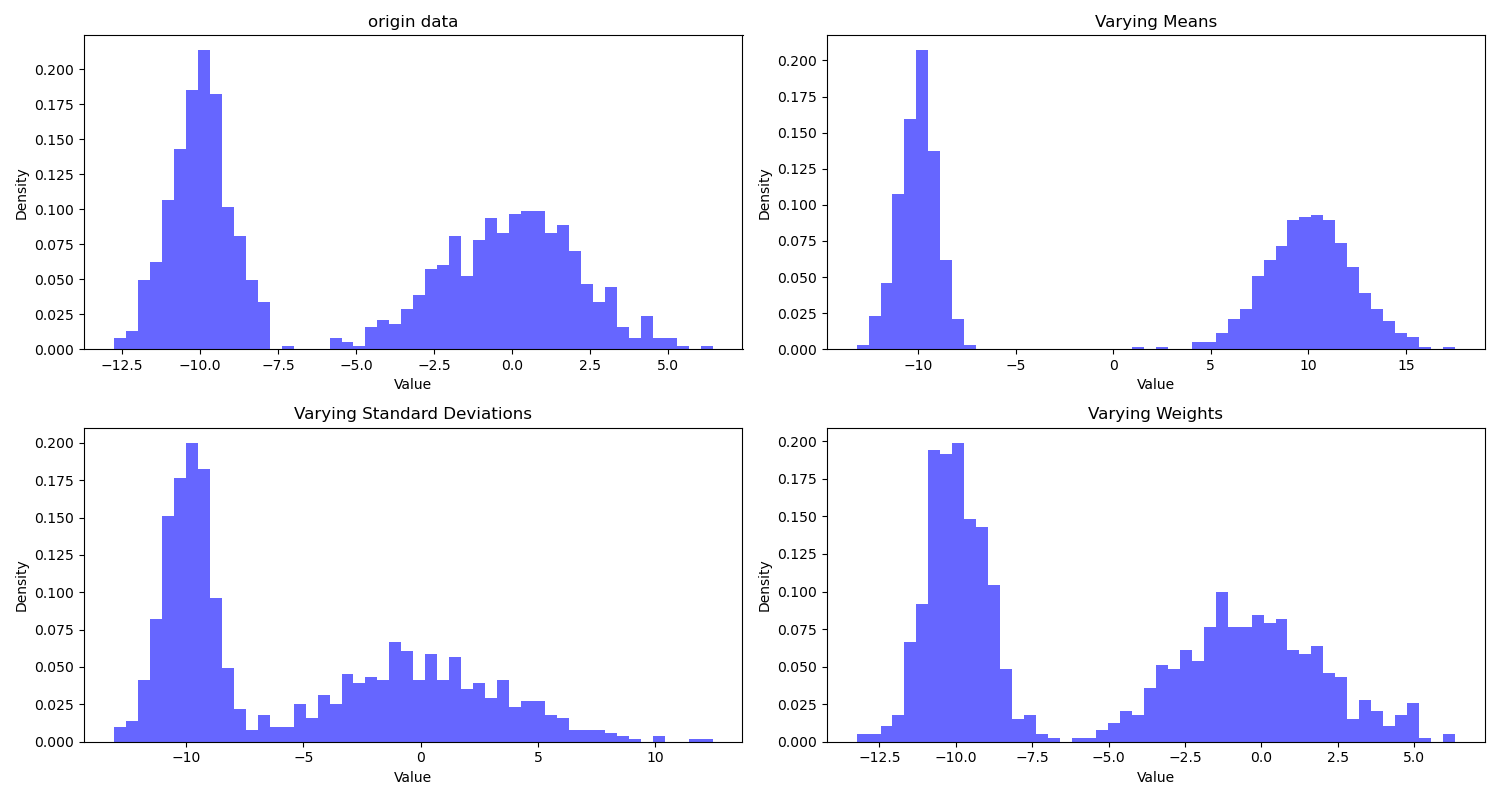
\includegraphics[width=0.8\textwidth,height=0.3\textwidth]{2.png}
  \caption{实验结果}
  \label{fig:my_label}
\end{figure}

在上图中展示了四个直方图,分别代表不同参数的变化,以下是对每个直方图的详细分析:

\paragraph{原始数据(左上图)}
此直方图展示了初始设定的混合高斯分布,呈现两个显著的峰值。这意味着存在两个不同的高斯分布组成部分,它们的均值相差较远,导致在值的分布上形成了两个中心。这种分布可能是由具有相对较小的标准差的两个高斯分布组合形成的,使得每个分布的数据点都相对集中在其各自的均值附近。


\paragraph{变化的均值(右上图)}
与左上角的原始数据图相比,这个直方图中的右侧峰值向右移动了,表明其中一个高斯分布的均值增大了。这导致了混合高斯分布中两个分布的右侧均值增大,从而产生一个向右偏的单一峰值。如果原始数据中两个高斯分布的均值相对较近,增大右侧分布的均值将使两个峰值拉开,但由于均值增大的分布可能具有更大的权重或者样本数更多,所以整体分布的峰值仍然表现出集中趋势。这种变化减少了两个分布间的重叠,使得混合分布的主要峰值偏向了均值增大的一侧。

\paragraph{变化的标准差(左下图)}
在这里,我们看到的是一个更为分散的分布,其中包括一个主要峰值和一个较小的峰值。增加一个高斯分布的标准差将导致数据点更广泛地分布在均值周围,从而使得直方图看起来更加扁平和宽敞。这表示分布中存在更大的变异性。

\paragraph{变化的权重(右下图)}
这个直方图显示了一个有两个峰,但不对称的分布。调整两个高斯分布的权重将改变它们在最终混合分布中的贡献。如果较小的峰值所对应的高斯分布权重减小,那么这个峰值在最终的混合分布中就不那么显著了。这个图展示了一个主峰和一个次峰,表明一个组分相对于另一个组分具有更大的权重。
\subsection{结论}
调整混合高斯分布的均值、方差(标准差)和系数(权重)会以不同的方式影响数据的分布。以下是每个参数调整对数据分布造成的影响:
\begin{list}
    \item 均值(Mean):
调整单个高斯分布的均值会改变该分布数据点的中心位置。
如果两个高斯分布的均值彼此接近,混合分布会倾向于表现出单峰特征。
如果均值相差很远,混合分布会表现出多峰特征,每个峰对应一个高斯分布的均值。
均值的变化也可以改变分布的对称性,特别是在不同高斯分布具有不同权重的情况下。

    \item 方差(Variance)/标准差(Standard Deviation):

方差或标准差的大小决定了单个高斯分布的数据点围绕其均值的散布程度。
较小的方差意味着数据点更集中,导致峰值更尖锐。
较大的方差意味着数据点更分散,导致峰值更平坦和更宽。
不同分布的方差差异可以导致混合分布中出现宽窄不一的峰值。

    \item 系数(Coefficient)/权重(Weight):

权重决定了单个高斯分布在混合分布中的相对重要性。
权重较大的分布在混合分布中更为显著,其特征(如峰值)在最终的混合分布中更加突出。
如果一个分布的权重被增加,混合分布的总体形状会更倾向于该分布的形状。
权重的调整还会影响混合分布中各个峰值的相对高度,进而影响整体分布的形状。
在实践中,通过细致地调整这些参数,可以控制混合高斯分布的整体形状,以模拟复杂的现实世界数据分布。例如,可以通过调整参数来拟合具有特定统计特性的实验数据,或者在机器学习中用于对特定数据集进行建模。

\end{list}





总结来说,改变混合高斯分布中的参数会导致数据分布的形状显著变化,这些变化反映了不同高斯组分对最终分布形状的不同影响。调整均值、标准差和权重参数可以控制分布的中心位置、分散程度和各组分的相对重要性,从而适应不同的数据分析需求。


\section{第二部分:中心极限定理的应用}

\subsection{代码解析}

第二份代码演示了中心极限定理(CLT)的应用。通过多次抽取样本并计算均值,可以观察到随着样本量的增加,样本均值的分布越来越接近正态分布。

\subsubsection{函数定义}
\begin{itemize}
  \item \texttt{generate\_mixed\_gaussian}: 与第一份代码中的同名函数功能相同。
  \item \texttt{problem2}: 该函数实现了 CLT 的模拟过程。它通过多次生成混合高斯分布的样本,计算样本均值,并绘制其分布的直方图。
\end{itemize}

\subsubsection{参数设置}

代码中预设了一个样本量列表 \texttt{nlist},其中包含从2到5000不等的样本量。通过改变样本量,可以观察样本均值分布的变化。

\subsection{结果分析}

\begin{figure}[h]
  \centering
  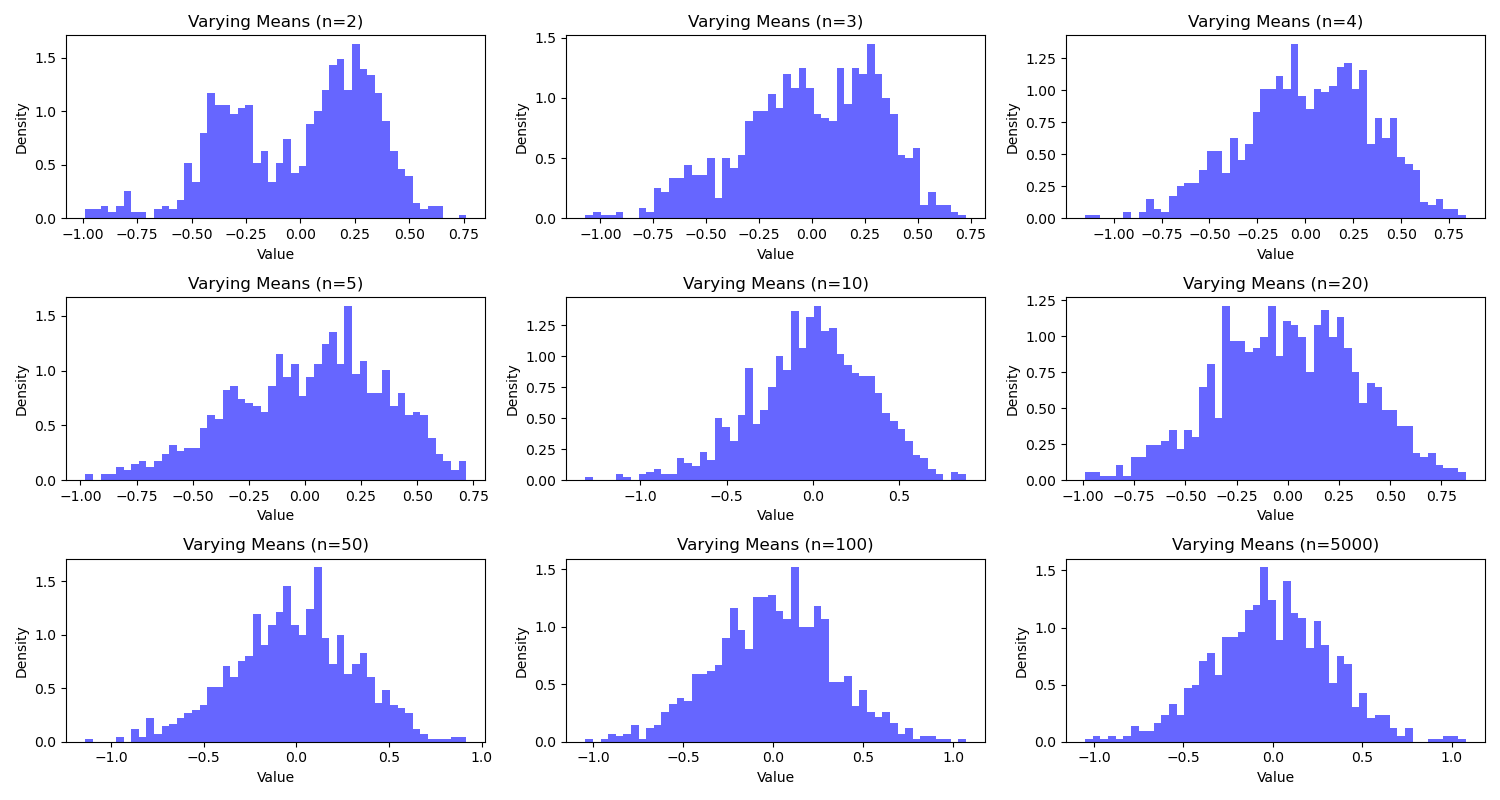
\includegraphics[width=0.8\textwidth,height=0.3\textwidth]{1.png}
  \caption{实验结果}
  \label{fig:my_label}
\end{figure}

在上图中,有一系列直方图展示了不同样本大小(n)的混合高斯分布的统计特性。从左上角到右下角,图像分别对应着样本大小为 2、3、4、5、10、20、50、100 和 5000 的情况。以下是对这些直方图的分析:

\paragraph{样本大小的影响}
直方图的形状变化揭示了样本大小(n)对估计混合高斯分布的影响。每个直方图反映了通过模拟混合高斯分布得到的统计量的分布,其中统计量通常是样本均值。

\paragraph{小样本大小(n=2, 3, 4, 5)}
对于较小的样本大小(n=2到5),直方图呈现出较多的随机性和不规则性。在n = 2时图像依然可以看到较为明显的两个峰值,这是因为当样本量很小时,随机性对结果的影响较大,因此样本倾向于表现为其本身的分布,图像可能会有所不同,导致统计量的分布看起来比较粗糙且不平滑。

\paragraph{中等样本大小(n=10, 20)}
当样本量增加到10和20时,直方图开始显现出更平滑且更接近正态分布的形状。中心极限定理(CLT)说明,即使原始数据不是正态分布的,样本均值的分布随着样本量的增加而趋向于正态分布。这里的直方图开始反映这一理论,峰值更加明显,且分布变得对称。

\paragraph{大样本大小(n=50, 100, 5000}
对于更大的样本量(n=50, 100,5000),直方图的形状变得非常平滑,并且明显呈现出了正态分布的特征,即单一的对称峰和两侧的尾部逐渐减少。这符合中心极限定理的预期,即样本均值将形成一个钟形的正态分布。对于n=5000的情况,直方图的形状几乎完美地符合正态分布的典型形态,表明了大数定律和中心极限定理在这里的应用。

\subsection{结论}
通过观察不同样本大小的混合高斯分布,我们可以看到,随着样本量的增加,样本均值的分布越来越趋于正态分布。这些直方图是中心极限定理在混合高斯分布上应用的直观展示。即使原始数据可能不是正态分布的,样本均值也会随着样本量的增加而趋近于正态分布。这一现象是统计学中非常重要的,因为它允许我们对大型样本集的性质进行推断,即使我们只能观察到来自该分布的有限样本。

\section{遇到的问题和解决方式}
\subsection{如何形成混合高斯分布}

\section{结论}

通过两份代码的分析与结果讨论,我们可以得出以下结论:

- 混合高斯分布可以通过调整均值、标准差和混合比例来控制分布的形状。
- 中心极限定理对于样本均值的分布具有普遍适用性。

本报告详细解析了两份 Python 代码的实现,并通过图形结果深入探讨了混合高斯分布和中心极限定理的性质。这些发现对于理解复杂数据分布具有重要意义,同时也展示了统计学在数据分析中的应用。

\end{document}

